%!TEX root = thesis.tex

\chapter{Introduction}

Timing behavior is one of the most important properties of computer systems. Especially in safety-critical applications, a wrong timed reaction of the system can have disastrous consequences, for example an intervention of pacemaker, that occurred too early or too late would risk the life of the patient. In Cyber-physical Systems, e.g. the Electronic Stability Control of a vehicle, wrong timing can also lead to property damage, injuries or deaths. Also environmental aspects are affected by timing cyber-physical systems, for example combustion engines need exact timing to produce as little emissions as possible.\\
The interconnection of several components in cyber-physical systems makes the design and analysis of the timing behavior of these systems significant hard, because not only the components on its own, but also the complete system must be considered. In this context, testing is a major problem, because it is hard to reproduce the exact state of the system, in which the error occurred. In many cases, the error does not lay in the component where it became visible, it was carried off to other parts, which results in a malfunctioning system, where it is extremely hard to find the bug that caused the problem. Online Monitoring is the key technique to address this problem, because you can isolate the error, without the need of storing and recreating the state of the system, when searching the error.\\
The goal of this thesis is to create a monitoring tool for the \emph{AUTOSAR} (\textbf{AUT}omotive \textbf{O}pen \textbf{S}ystem \textbf{AR}chitecture) Timing Extensions, which were created to increase the interoperability and exchangeability of car components.

\section{AUTOSAR TIMEX}
AUTOSAR is a development partnership in the automotive industry. As stated before, the main goal is to define a standardized interface, to increase interoperability, exchangebility and re-usability of parts and therefore simplify development and production. Three different layers are defined in the specification. \emph{Basic Software} is an abstraction layer from components, like network or diagnostic protocols, or operating systems. \emph{AUTOSAR-Software} defines, how application has to be build. For Basic Software and AUTOSAR Software, there are definitions for standardized Interfaces, to enable the communication via the \emph{Autosar Runtime Environment}. It works as middleware, in which the \emph{virtual function bus} is defined ~\cite{Virtual_Functional_Bus}.
The AUTOSAR Timing Extension are describing timing constraints for actions and reactions of components, that are communicating via the Virtual Function Bus, for example the latency timing constraint, that describes the amount of time between two subsequent events, or the event triggering constraints, that are used to describe the timing behavior of events, that are created in one component without getting input from another component.\\
Problematic with the AUTOSAR Timing Extensions is, that the definitions are not very formal and have room left for interpretation. Let's take a look at the \emph{BurstPatternEventTriggering}. The BurstPatternEventTriggerings describe events clusters, with events that occur with short time distances, with large time distances between the clusters. The following attributes are needed:\\ \\
\begin{tabular}{|c|c|c|}
	\hline
	\textbf{Attribute} & \textbf{Type} & \textbf{Explanation} \\
	\hline
	$maxNumberOfOccurrences$ & PositiveInteger & maximum number of events per burst\\
	\hline
	$minNumberOfOccurrences$ & PositiveInteger & (optional) minimum number of\\
						   &				 & events per burst\\
	\hline
	$minimumInterArrivalTime$ & TimeValue & minimum time distance between any\\
							&			& two events\\
	\hline
	$patternLength$ & TimeValue &  length of each burst\\
	\hline
	$patternPeriod$ & TimeValue & (optional) Time distance between the\\
	 			  &			  & start points of two subsequent bursts\\
	\hline
	$patternJitter$ & TimeValue & (optional) maximum of allowed\\
    			  &			  & deviation from periodic pattern\\
	\hline
\end{tabular}\\ \\ \\
As example, we set:
\begin{itemize}
	\item
		$maxNumberOfOccurrences = 3$
	\item
		$minNumberOfOccurrences = 1$
	\item
		$minimumInterArrivalTime = 1$
	\item
		$patternLength = 3$
	\item
		$patternPeriod = 3.5$
	\item
		$patternJitter = 1.5$
\end{itemize}

\begin{figure}
	\centering
	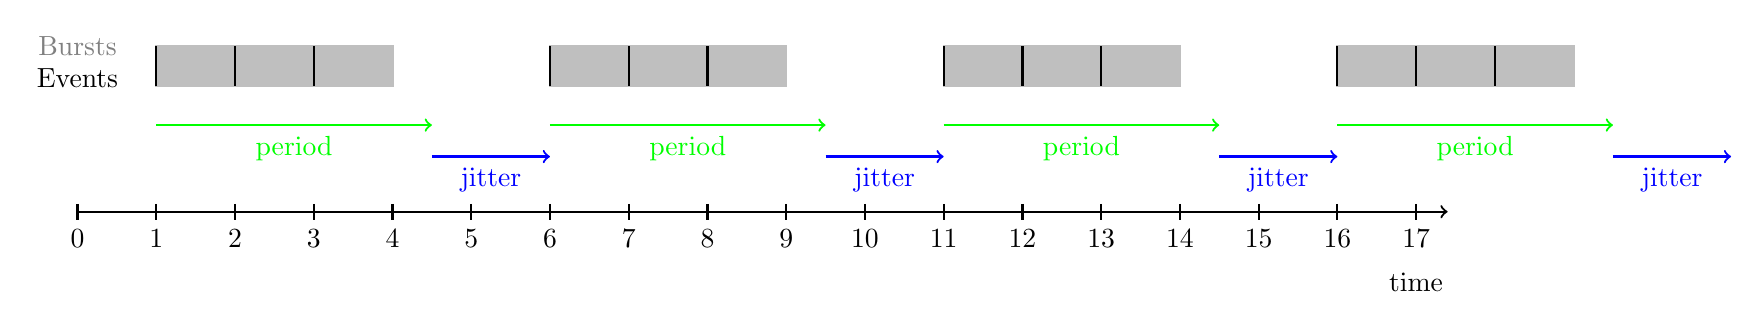
\begin{tikzpicture}[thick]
		% time axis
		\foreach \x in {0,...,17}
			\draw (\x,-4) -- (\x,-4.2) node[anchor=north] {\x};
		\draw[->] (0, -4.1) -- (17.4, -4.1);
		\node at(17, -5) {time};
		
		% bursts
		\node[gray] at (0, -2){Bursts};
		\draw [fill=lightgray, lightgray] (1, -2) rectangle (4,-2.5);
		\draw [fill=lightgray, lightgray] (6, -2) rectangle (9,-2.5);
		\draw [fill=lightgray, lightgray] (11, -2) rectangle (14,-2.5);
		\draw [fill=lightgray, lightgray] (16, -2) rectangle (19,-2.5);
		% events
		\node at (0, -2.4){Events};
		%\node at (0, -2.15){events};
		\foreach \x in {1, 6, 11, 16}
		{
			% events
			\draw[-] (\x, -2) -- (\x, -2.5);
			\draw[-] (\x+1, -2) -- (\x+1, -2.5);
			\draw[-] (\x+2, -2) -- (\x+2, -2.5);
			% periods
			\draw[->, green] (\x, -3) -- (\x+3.5, -3);
			\node[green] at (\x+1.75, -3.3){period};
			%jitters
			\draw[->, blue] (\x+3.5,-3.4) -- (\x+5, -3.4);
			\node[blue] at (\x+4.25, -3.7) {jitter};
		}
	\end{tikzpicture}
	\caption{BurstPatternEventTriggering Period-Jitter \textbf{accumulating}}
	\label{fig:BurstPatternEventTriggering1}
\end{figure}
\begin{figure}
	\centering
	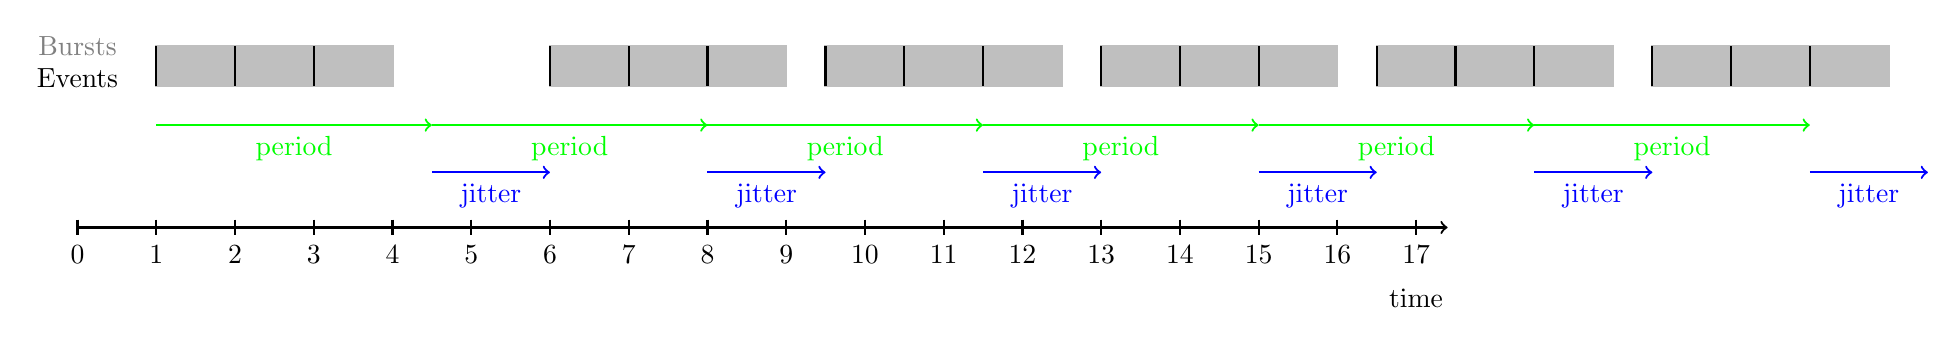
\begin{tikzpicture}[thick]
	% time axis
	\foreach \x in {0,...,17}
	\draw (\x,-4.2) -- (\x,-4.4) node[anchor=north] {\x};
	\draw[->] (0, -4.3) -- (17.4, -4.3);
	\node at(17, -5.2) {time};
	
	% bursts
	\node[gray] at (0, -2){Bursts};
	\draw [fill=lightgray, lightgray] (1, -2) rectangle (4,-2.5);
	\node at (0, -2.4){Events};
	
	%period 1
	\draw[->, green] (1, -3) -- (4.5, -3);
	\node[green] at (2.75, -3.3){period};
	
	% jitter 1
	\draw[->, blue] (4.5,-3.6) -- (6, -3.6);
	\node[blue] at (5.25, -3.9) {jitter};
	
	\foreach \y in {0, 1, 2}
		\draw[-] (1+\y, -2) -- (1+\y, -2.5);
	
	\foreach \x in {4.5, 8, 11.5, 15, 18.5}
	{
		% periods
		\draw[->, green] (\x, -3) -- (\x+3.5, -3);
		\node[green] at (\x+1.75, -3.3){period};
		% jitters
		\draw[->, blue] (\x+3.5,-3.6) -- (\x+5, -3.6);
		\node[blue] at (\x+4.25, -3.9) {jitter};
		%bursts	
		\draw [fill=lightgray, lightgray] (\x+1.5, -2) rectangle (\x+4.5,-2.5);
		% events
		\foreach \y in {0, 1, 2}
			\draw[-] (\x+\y+1.5, -2) -- (\x+\y+1.5, -2.5);
	}
	\end{tikzpicture}
	\caption{BurstPatternEventTriggering Period-Jitter \textbf{non-accumulating}}
	\label{fig:BurstPatternEventTriggering2}
\end{figure}

The combination of $patternPeriod$ and $patternJitter$ can be interpreted in an accumulating as seen in \ref{fig:BurstPatternEventTriggering1} or non-accumulating way as seen in \ref{fig:BurstPatternEventTriggering2} way. In the accumulating interpretation, the reference for the periodic occurrences is only the start point of the previous 

With the definition of $patternLength$ (\glqq time distance between the beginnings of subsequent repetitions of the given burst pattern\grqq) you would think, that the accumulating variant is meant. Against that, the period attribute in $PeriodicEventTriggering$-Constraint is also defined as \glqq distance between subsequent occurrences of the event\grqq in the text, hence it is understandable the accumulating way, but there is also the formal definition

\begin{math}
	\exists t_{reference}\forall t_n: t_{reference}+(n+1)*period\leq t_n\leq t_{reference}+(n-1)*period+jitter,
\end{math}

where $t_n$ is the time of the $n$-th Event and $t_{reference}$ is a reference point, from which the periodic pattern starts, so the $PeriodicEventTriggering$-Constraint is meant to be understood in the non-accumulating way. It remains unclear, in which way the $BurstPatternEventTriggering$ is meant to be understood.

Another problem of the AUTOSAR Timing Extensions is, that they were made for design purposes, monitoring them can be difficult, as they may need continuously growing time and memory resources, which makes online monitoring impossible (more on monitorability in \ref{chapter-monitorability}). As example, we will use the burst pattern again, this time using the attributes as
\begin{itemize}
	\item
		$maxNumberOfOccurrences = 100$
	\item
		$minNumberOfOccurrences = 1$
	\item
		$minimumInterArrivalTime = 0$
	\item
		$patternLength = 3$
	\item
		\textcolor{gray}{$patternPeriod$ unused}
	\item
		\textcolor{gray}{$patternJitter$ unused}
\end{itemize}
\begin{figure}
	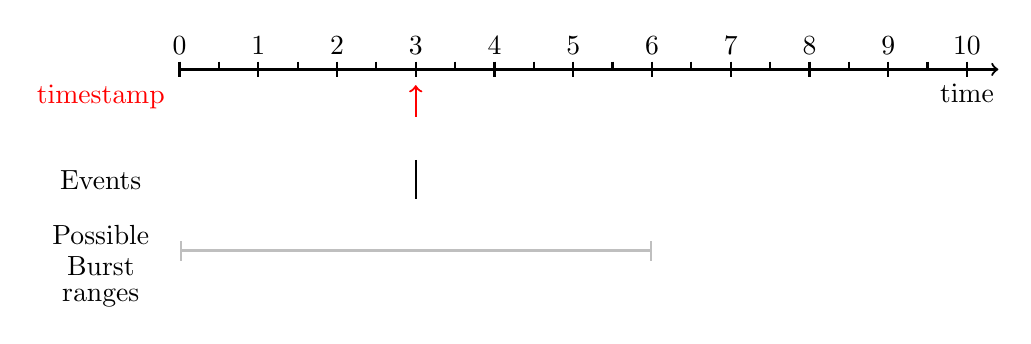
\begin{tikzpicture}[thick]
		%time axis
		\foreach \x in {0,...,10}
		{
			\draw (\x,0) -- (\x,-0.2);
			\node at (0+\x, 0.2) {\x};
		}
		\foreach \x in {0,...,9}
			\draw (\x+0.5,0) -- (\x+0.5,-0.1);
		\draw[->] (0, -0.1) -- (10.4, -0.1);
		\node at(10, -0.4) {time};
		
		\node[red] at(-1, -0.45) {timestamp};
		%watched time
		\draw[->, red] (3, -0.7)--(3, -0.3);
		
		\node at (-1, -1.5) {Events};
		\draw[-] (3, -1.25) -- (3, -1.75);
		
		\node at (-1, -2.2) {Possible};
		\node at (-1, -2.6) {Burst};
		\node at (-1, -3) {ranges};
		
		%Burst range
		\draw[|-|, lightgray] (0, -2.4) -- (6, -2.4);
	\end{tikzpicture}
	
	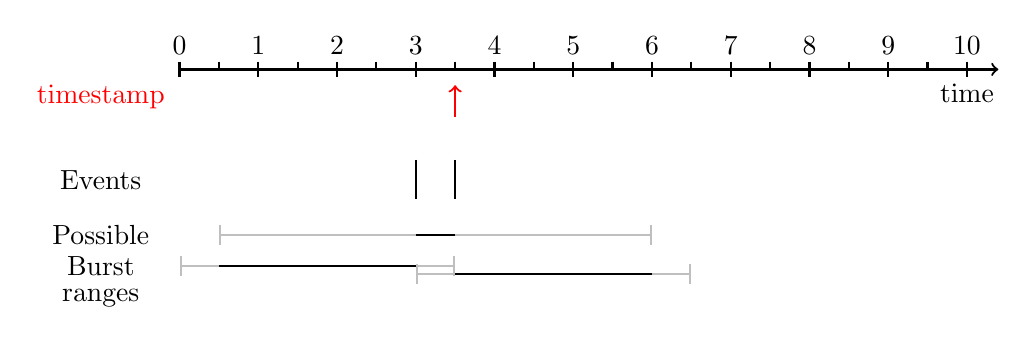
\begin{tikzpicture}[thick]
		%time axis
		\foreach \x in {0,...,10}
		{
			\draw (\x,0) -- (\x,-0.2);
			\node at (0+\x, 0.2) {\x};
		}
		\foreach \x in {0,...,9}
			\draw (\x+0.5,0) -- (\x+0.5,-0.1);
		\draw[->] (0, -0.1) -- (10.4, -0.1);
		\node at(10, -0.4) {time};
		
		\node[red] at(-1, -0.45) {timestamp};
		%watched time
		\draw[->, red] (3.5, -0.7)--(3.5, -0.3);
		
		\node at (-1, -1.5) {Events};
		\draw[-] (3, -1.25) -- (3, -1.75);
		\draw[-] (3.5, -1.25) -- (3.5, -1.75);
		
		\node at (-1, -2.2) {Possible};
		\node at (-1, -2.6) {Burst};
		\node at (-1, -3) {ranges};
		
		%Burst range 1
		\draw[|-|, lightgray] (0.5, -2.2) -- (6, -2.2);
		\draw[-] (3, -2.2) -- (3.5, -2.2);
		% Burst range 2
		\draw[|-|, lightgray] (0, -2.6) -- (3.5, -2.6);
		\draw[-] (0.5, -2.6) -- (3, -2.6);
		\draw[|-|, lightgray] (3, -2.7) -- (6.5, -2.7);
		\draw[-] (3.5, -2.7) -- (6, -2.7);
	\end{tikzpicture}
	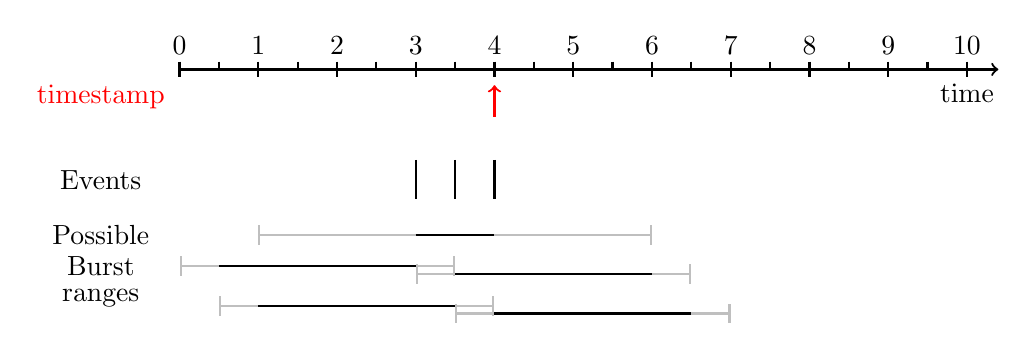
\begin{tikzpicture}[thick]
		%time axis
		\foreach \x in {0,...,10}
		{
			\draw (\x,0) -- (\x,-0.2);
			\node at (0+\x, 0.2) {\x};
		}
		\foreach \x in {0,...,9}
		\draw (\x+0.5,0) -- (\x+0.5,-0.1);
		\draw[->] (0, -0.1) -- (10.4, -0.1);
		\node at(10, -0.4) {time};
		
		\node[red] at(-1, -0.45) {timestamp};
		%watched time
		\draw[->, red] (4, -0.7)--(4, -0.3);
		
		\node at (-1, -1.5) {Events};
		\draw[-] (3, -1.25) -- (3, -1.75);
		\draw[-] (3.5, -1.25) -- (3.5, -1.75);
		\draw[-] (4, -1.25) -- (4, -1.75);
		
		\node at (-1, -2.2) {Possible};
		\node at (-1, -2.6) {Burst};
		\node at (-1, -3) {ranges};
		
		%Burst ranges poss. 1
		\draw[|-|, lightgray] (1, -2.2) -- (6, -2.2);
		\draw[-] (3, -2.2) -- (4, -2.2);
		% Burst ranges poss. 3 2.6,2.7
		\draw[|-|, lightgray] (0, -2.6) -- (3.5, -2.6);
		\draw[-] (0.5, -2.6) -- (3, -2.6);
		\draw[|-|, lightgray] (3, -2.7) -- (6.5, -2.7);
		\draw[-] (3.5, -2.7) -- (6, -2.7);
		% Burst ranges poss. 2
		\draw[|-|, lightgray] (0.5, -3.1) -- (4, -3.1);
		\draw[-] (1, -3.1) -- (3.5, -3.1);
		\draw[|-|, lightgray] (3.5, -3.2) -- (7, -3.2);
		\draw[-] (4, -3.2) -- (6.5, -3.2);
	\end{tikzpicture}
		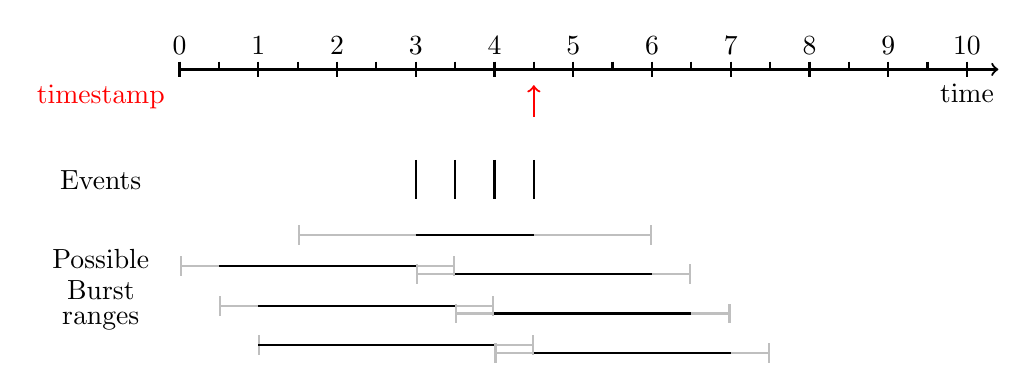
\begin{tikzpicture}[thick]
		%time axis
		\foreach \x in {0,...,10}
		{
			\draw (\x,0) -- (\x,-0.2);
			\node at (0+\x, 0.2) {\x};
		}
		\foreach \x in {0,...,9}
		\draw (\x+0.5,0) -- (\x+0.5,-0.1);
		\draw[->] (0, -0.1) -- (10.4, -0.1);
		\node at(10, -0.4) {time};
		
		\node[red] at(-1, -0.45) {timestamp};
		%watched time
		\draw[->, red] (4.5, -0.7)--(4.5, -0.3);
		
		\node at (-1, -1.5) {Events};
		\draw[-] (3, -1.25) -- (3, -1.75);
		\draw[-] (3.5, -1.25) -- (3.5, -1.75);
		\draw[-] (4, -1.25) -- (4, -1.75);
		\draw[-] (4.5, -1.25) -- (4.5, -1.75);
		
		\node at (-1, -2.5) {Possible};
		\node at (-1, -2.9) {Burst};
		\node at (-1, -3.3) {ranges};
		
		%Burst ranges poss. 1
		\draw[|-|, lightgray] (1.5, -2.2) -- (6, -2.2);
		\draw[-] (3, -2.2) -- (4.5, -2.2);
		% Burst ranges poss. 2
		\draw[|-|, lightgray] (0, -2.6) -- (3.5, -2.6);
		\draw[-] (0.5, -2.6) -- (3, -2.6);
		\draw[|-|, lightgray] (3, -2.7) -- (6.5, -2.7);
		\draw[-] (3.5, -2.7) -- (6, -2.7);
		% Burst ranges poss. 3
		\draw[|-|, lightgray] (0.5, -3.1) -- (4, -3.1);
		\draw[-] (1, -3.1) -- (3.5, -3.1);
		\draw[|-|, lightgray] (3.5, -3.2) -- (7, -3.2);
		\draw[-] (4, -3.2) -- (6.5, -3.2);
		% Burst ranges poss. 4
		\draw[|-|, lightgray] (1, -3.6) -- (4.5, -3.6);
		\draw[-] (1, -3.6) -- (4, -3.6);
		\draw[|-|, lightgray] (4, -3.7) -- (7.5, -3.7);
		\draw[-] (4.5, -3.7) -- (7, -3.7);
	\end{tikzpicture}
\end{figure}


%\section{Verwandte Arbeiten}
 
%\textbf{AUTOSAR} (AUTomotive Open System ARchitecture) ist eine Partnerschaft aus Automobilherstellern und dazugehörigen Software, Hardware Unternehmen, deren Zulieferern und weiteren. Ziel dieser Partnerschaft ist die Erstellung offener Standards für Soft- und Hardwarekomponenten im Automobilbereich, sowie deren Entwicklungsprozesse ~\cite{AUTOSAR_History}.\\
%Die AUTOSAR Timing Extensions (kurz \textbf{AUTOSAR TIMEX}) spezifieren Constraints, mit denen das Zeitverhalten von Komponenten, die mit Hilfe anderer AUTOSAR Standards definiert wurden, beschrieben werden kann ~\cite{TIMEX}.\\
%TODO ~\cite{TIMMO2USE}\\
%\textbf{TeSSLa} (Temporal Stream-based Specification Language) ist eine turingfähige Programmiersprache, die zur Analyse und zur Überwachung von Zeitverhalten, insbesondere das von Cyber-Physical Systems. Es nimmt dabei Ströme von Datenpunkten, die mit Zeitstempeln verknüpft sind, entgegen und führt auf diesen Berechnungen durch ~\cite{TeSSLa}.\\
%Damit eng verknüpft ist das \textbf{COEMS}-Project, in dem Möglichkeiten von hardwarebasierte, non-intrusive, online Stream Runtime Verification erarbeitet wurden. Hierbei werden vorhandene Debug-Informationen aus einem System mittels einer TeSSLa-Spezifikation, die auf eine FPGA-basierter Hardware übertragen wurde, analysiert.



% Eine wichtiger Abschnitt der Einleitung stellt einen Überblick über verwandte Arbeiten dar. Was wurde bereits in der Literatur untersucht und ist \emph{nicht} Thema dieser Arbeit?

%\section{Aufbau der Arbeit}

%Neben dieser Einleitung und der Zusammenfassung am Ende gliedert sich diese Arbeit in die folgenden drei Kapitel.
%\begin{description}
%  \item[\ref{chapter-basics}] beschreibt die für diese Arbeit benötigten Grundlagen. In diesem Kapitel werden \ldots, \ldots und \ldots eingeführt, da diese für die folgenden Kapitel dringend benötigt werden.
%  \item[\ref{chapter-konzept}] stellt das eigentliche Konzept vor. Dabei handelt es sich um ein Konzept zur Verbesserung der Welt. Das Kapitel gliedert sich daher in einen globalen und einen lokalen Ansatz, wie die Welt zum Besseren beeinflusst werden kann.
%  \item[\ref{chapter-evaluation}] beinhaltet eine Evaluation des Konzeptes aus dem vorherigen Kapitel. Anhand von Simulationen wird in diesem Kapitel untersucht, wie die Welt durch konkrete Maßnahmen deutlich verbessert werden kann.
%\end{description}

